% Chapter Template

\chapter{Chapter Title Here}\label{chapter:firstchapter} % Main chapter title

\label{ChapterX} % Change X to a consecutive number; for referencing this chapter elsewhere, use \ref{ChapterX}

%----------------------------------------------------------------------------------------
%	SECTION 1
%----------------------------------------------------------------------------------------

\section{Main Section 1}\label{sec:firstsection}

% It is a good idea to have each sentence on a separate line, so that if you get feedback or changes from someone else
% the diffs will be much easier to manage
Lorem ipsum dolor (Figure \ref{fig:ThisFig}) sit amet, consectetur adipiscing elit\cite{fleischman1994pragmatics}.
Aliquam ultricies lacinia euismod.
Nam tempus risus in dolor rhoncus in interdum enim tincidunt.
Donec vel nunc (Figure \ref{fig:CheeseFig}) neque \cite{lawless1995multidimensional}.
In condimentum ullamcorper quam non consequat.
Fusce sagittis tempor feugiat.
Fusce magna erat, molestie eu convallis ut, tempus sed arcu.
Quisque molestie, ante a tincidunt ullamcorper, sapien enim dignissim lacus, in semper nibh erat lobortis purus.
Integer dapibus ligula ac risus convallis pellentesque.


\begin{figure}
\begin{centering}
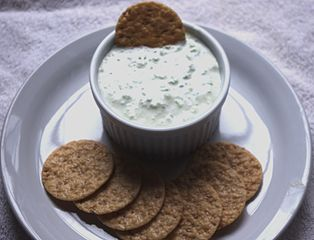
\includegraphics[width=10cm,height=10cm,keepaspectratio]{Figures/cheese.jpg}
\caption{Some cheese. Image Credit Geoff Lane (License: CC3-A-SA)}
\label{fig:CheeseFig}
\end{centering}
\end{figure}


\begin{figure}
\begin{centering}
\includegraphics[width=10cm,height=10cm,keepaspectratio]{Figures/dont-panic-e1534046233310.jpg}
\caption{The Hitch Hiker's Guide To The Galaxy (not to be confused with \cite{Reference1}. Image Credit David Strine (License: CC0)}
\label{fig:ThisFig}
\end{centering}
\end{figure}

%-----------------------------------
%	SUBSECTION 1
%-----------------------------------
\subsection{Subsection 1}

Nunc posuere quam at lectus tristique eu ultrices augue venenatis (Chapter \ref{chapter:firstchapter}).
Vestibulum ante ipsum primis in faucibus orci luctus et ultrices posuere cubilia Curae; Aliquam erat volutpat.
Vivamus sodales tortor eget quam adipiscing in vulputate ante ullamcorper.
Sed eros ante, lacinia et sollicitudin et, aliquam sit amet augue.
In hac habitasse platea dictumst (Section \ref{sec:firstsection}).

%-----------------------------------
%	SUBSECTION 2
%-----------------------------------

\subsection{Subsection 2}
Morbi rutrum odio eget arcu adipiscing sodales.
Aenean et purus a est pulvinar pellentesque.
 Cras in elit neque, quis varius elit.
 Phasellus fringilla, nibh eu tempus venenatis, dolor elit posuere quam, quis adipiscing urna leo nec orci.
 Sed nec nulla auctor odio aliquet consequat.
 Ut nec nulla in ante ullamcorper aliquam at sed dolor.
 Phasellus fermentum magna in augue gravida cursus.
 Cras sed pretium lorem.
 Pellentesque eget ornare odio.
 Proin accumsan, massa viverra cursus pharetra, ipsum nisi lobortis velit, a malesuada dolor lorem eu neque.

%----------------------------------------------------------------------------------------
%	SECTION 2
%----------------------------------------------------------------------------------------

\section{Main Section 2}

Sed ullamcorper quam eu nisl interdum at interdum enim egestas.
 Aliquam placerat justo sed lectus lobortis ut porta nisl porttitor.
 Vestibulum mi dolor, lacinia molestie gravida at, tempus vitae ligula.
 Donec eget quam sapien, in viverra eros.
 Donec pellentesque justo a massa fringilla non vestibulum metus vestibulum.
 Vestibulum in orci quis felis tempor lacinia.
 Vivamus ornare ultrices facilisis.
 Ut hendrerit volutpat vulputate.
 Morbi condimentum venenatis augue, id porta ipsum vulputate in.
 Curabitur luctus tempus justo.
 Vestibulum risus lectus, adipiscing nec condimentum quis, condimentum nec nisl.
 Aliquam dictum sagittis velit sed iaculis.
 Morbi tristique augue sit amet nulla pulvinar id facilisis ligula mollis.
 Nam elit libero, tincidunt ut aliquam at, molestie in quam.
 Aenean rhoncus vehicula hendrerit.
